\documentclass[titlepage]{article}
\usepackage{graphicx}
\usepackage{fancyhdr}
\usepackage{hyperref}

\title{Computer Workshop Final Project}
\author{SeyedAli Hoseini}
\date{5 Bahman 1402}

\pagestyle{fancy}

\begin{document}
\maketitle
\tableofcontents

\newpage

\section{Git and GitHub}
\subsection{Repository Initialization and Commits}
At first, I created the repository on GitHub using the "New Repository" button. After that, I cloned it using "git clone." Then, I added configurations following the instructions, created the main LaTeX file, and committed and pushed these changes.

\subsection{GitHub Actions for LaTeX Compilation}
First of all, I created the relevant file in the address associated with the workflows and copied its content from the repository provided for guidance. However, it seemed that the compilation to PDF was not working. But I didn't give up, and by visiting the provided link, I copied the file content from there, and apparently, it worked well after that.

\newpage

\section{Exploration Tasks}
\subsection{Vim Advanced Features}
\begin{enumerate}
    \item Regular Expressions and Search Patterns\\
    Vim supports powerful regular expressions for search and replace operations. You can create complex search patterns to find and manipulate text efficiently.

    \item Registers and Shell Integration\\
    Vim's registers not only store yanked or deleted text but also allow you to interact with the system shell. You can execute shell commands from within Vim, capture their output, and even paste the output directly into your document.

    \item Autocompletion and IntelliSense\\
    Vim supports autocompletion for code, making coding faster and more accurate. Plugins like YouCompleteMe or coc.nvim provide IntelliSense-like features, offering suggestions for code completion, function signatures, and documentation as you type.
\end{enumerate}
\subsection{Memory profiling}
\subsubsection{Memory Leak}
Memory leaks occur when a computer program allocates memory for an object or data but fails to release or deallocate that memory when it's no longer needed. This leads to a gradual increase in the program's memory usage over time. Memory leaks can happen in a program when developers forget to free up memory, causing it to accumulate and potentially degrade the performance of the application. Common causes include not releasing allocated memory, circular references, and incorrectly implemented data structures.
\subsubsection{Memory profilers}
Valgrind is a programming tool designed for memory debugging, memory leak detection, and profiling. It is widely used for analyzing and identifying memory-related issues in C and C++ programs. It actively detects instances where memory is allocated but not properly deallocated during program execution. Through detailed reports, Valgrind highlights the exact lines of code responsible for memory leaks and provides call stack information, aiding developers in understanding the sequence of function calls leading to the allocation.
\subsection{GNU/Linux Bash Scripting}
\subsubsection{fzf}
\begin{enumerate}
    \item Fuzzy searching is a method that finds approximate matches for a query, accommodating typos or variations in text. It's useful when exact matches may not be available, allowing systems to retrieve relevant results based on similarity rather than strict matching.

    \item This command lists files and directories using "ls" and then pipes the output into "fzf," enabling us to search the results of "ls".
\end{enumerate}
\subsubsection{Using fzf to find your favorite PDF}
\begin{verbatim}
fd -e pdf
fd -e pdf | fzf
\end{verbatim}
\subsubsection{Opening the file using Zathura}
\begin{verbatim}
zathura "$(fd -e pdf | fzf)"
\end{verbatim}
\newpage
\section{Git and FOSS}
\subsection{README.md}
You can find detailed information about the project in the \href{https://github.com/sseeyyeedd/CW-Final-Project/blob/main/README.md}{README.md} file.

\subsection{Issues}
\begin{figure}[ht]
    \centering
    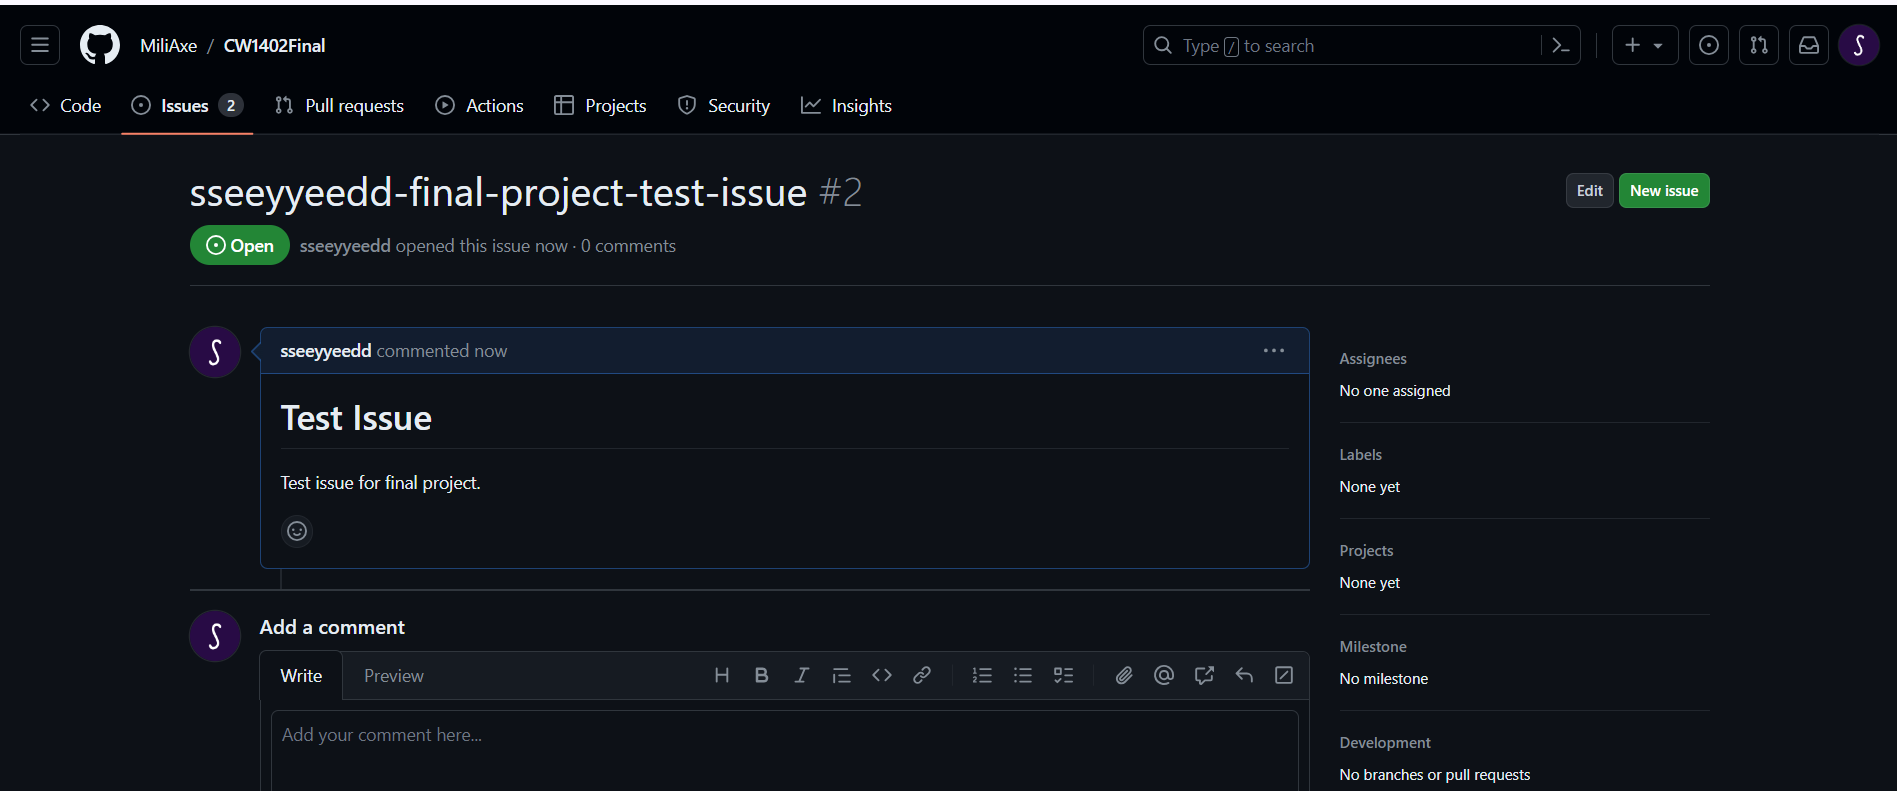
\includegraphics[width=1\textwidth]{s.png}
    \caption{Issue screenshot}
\end{figure}
\end{document}

